
\documentclass{beamer}

%\usepackage[table]{xcolor}
\mode<presentation> {
  \usetheme{Boadilla}

%  \usetheme{Pittsburgh}
%\usefonttheme[2]{sans}
\renewcommand{\familydefault}{cmss}
%\usepackage{lmodern}
%\usepackage[T1]{fontenc}
%\usepackage{palatino}
%\usepackage{cmbright}
 
\useinnertheme{rectangles}
}

\setbeamercolor{normal text}{fg=black}
\setbeamercolor{structure}{fg= blue}
\definecolor{trial}{cmyk}{1,0,0, 0}
\definecolor{trial2}{cmyk}{0.00,0,1, 0}
\definecolor{darkgreen}{rgb}{0,.4, 0.1}
\usepackage{array}
\beamertemplatesolidbackgroundcolor{white}  \setbeamercolor{alerted
text}{fg=red}
\usepackage{tcolorbox}
\setbeamertemplate{caption}[numbered]\newcounter{mylastframe}


\usepackage{tikz}
\usetikzlibrary{arrows}
\usepackage{colortbl}

\renewcommand{\familydefault}{cmss}
%\usepackage[all]{xy}

\usepackage{tikz}
\usepackage{lipsum}

 \newenvironment{changemargin}[3]{%
 \begin{list}{}{%
 \setlength{\topsep}{0pt}%
 \setlength{\leftmargin}{#1}%
 \setlength{\rightmargin}{#2}%
 \setlength{\topmargin}{#3}%
 \setlength{\listparindent}{\parindent}%
 \setlength{\itemindent}{\parindent}%
 \setlength{\parsep}{\parskip}%
 }%
\item[]}{\end{list}}
\usetikzlibrary{arrows}

\usecolortheme{lily}

\newtheorem{com}{Comment}
\newtheorem{lem} {Lemma}
\newtheorem{prop}{Proposition}
\newtheorem{condition}{Condition}
\newtheorem{thm}{Theorem}
\newtheorem{defn}{Definition}
\newtheorem{cor}{Corollary}
\newtheorem{obs}{Observation}
 \numberwithin{equation}{section}
 

\setbeamertemplate{navigation symbols}{}


\title[PLSC 43401]{Mathematical Foundations of Political Methodology}

\author{Robert Gulotty}
\institute[Chicago]{University of Chicago}
\vspace{0.3in}



\begin{document}

\begin{frame}
\maketitle
\end{frame}
\begin{frame}
\frametitle{What is this half of the course about?}
\begin{itemize}
\item The science of describing uncertainty
\item How to separate the signal from the noise
\item More problem solving with computers
\end{itemize}
\end{frame}






\begin{frame}{Origins of Probability Theory}

In 1717, gamblers played a dice game in which you would make the following bet:
\begin{tcolorbox}
\textbf{Bet A} At least one `1' will appear in a total of four rolls of a die.\\
\end{tcolorbox}
\pause
\begin{itemize}
\item \emph{Antoine Gombaud, Chevalier de M\'{e}r\'{e}} proposed a tougher game, rolling \emph{two} die, looking for a pair of `1'.\\
\pause
\item He figured, for a single trial, the chance of getting two `1` was one 1/6th as likely as one `1` : \pause
\item[$\rightarrow$] P( two `1`) =  P(one `1')$\times\frac{1}{6}$
\pause
\item One sixth as likely?  Maybe multiply the four rolls by six.
\pause  
\end{itemize}
\begin{tcolorbox}
\textbf{Bet B}  At least one pair of `1' will appear in a total of 24 rolls of two dice.
\end{tcolorbox}
\end{frame}

\begin{frame}{Origins of Probability Theory}

\begin{itemize}
\item Over the course of his holiday, the Chevalier de M\'{e}r\'{e} tried his bets on his friends 
\item Bet A worked quite well, Antoine would get a `1' in four rolls of a die more often than not. \pause
\item Bet B was working worse. His friends were winning more than he was losing.
\end{itemize}
\end{frame}

\begin{frame}[fragile]
\begin{verbatim}
> 1:6  # Sample space of a single die
[1] 1 2 3 4 5 6

> sample(1:6, size = 4, replace=TRUE)
[1] 4 4 2 2

> onedice4x <- replicate( n = 1000, 
sample(1:6, size = 4, replace=TRUE))

> n_ones <- colSums( onedice4x == 1)

> table(n_ones>0) # Bet A outcomes:

FALSE  TRUE 
  480   520 
 
\end{verbatim}
\end{frame}

\begin{frame}[fragile]
\begin{verbatim}
> plot(cumsum(n_ones>0)/1:1000, cex=.2)
> abline(h=.5)
\end{verbatim}

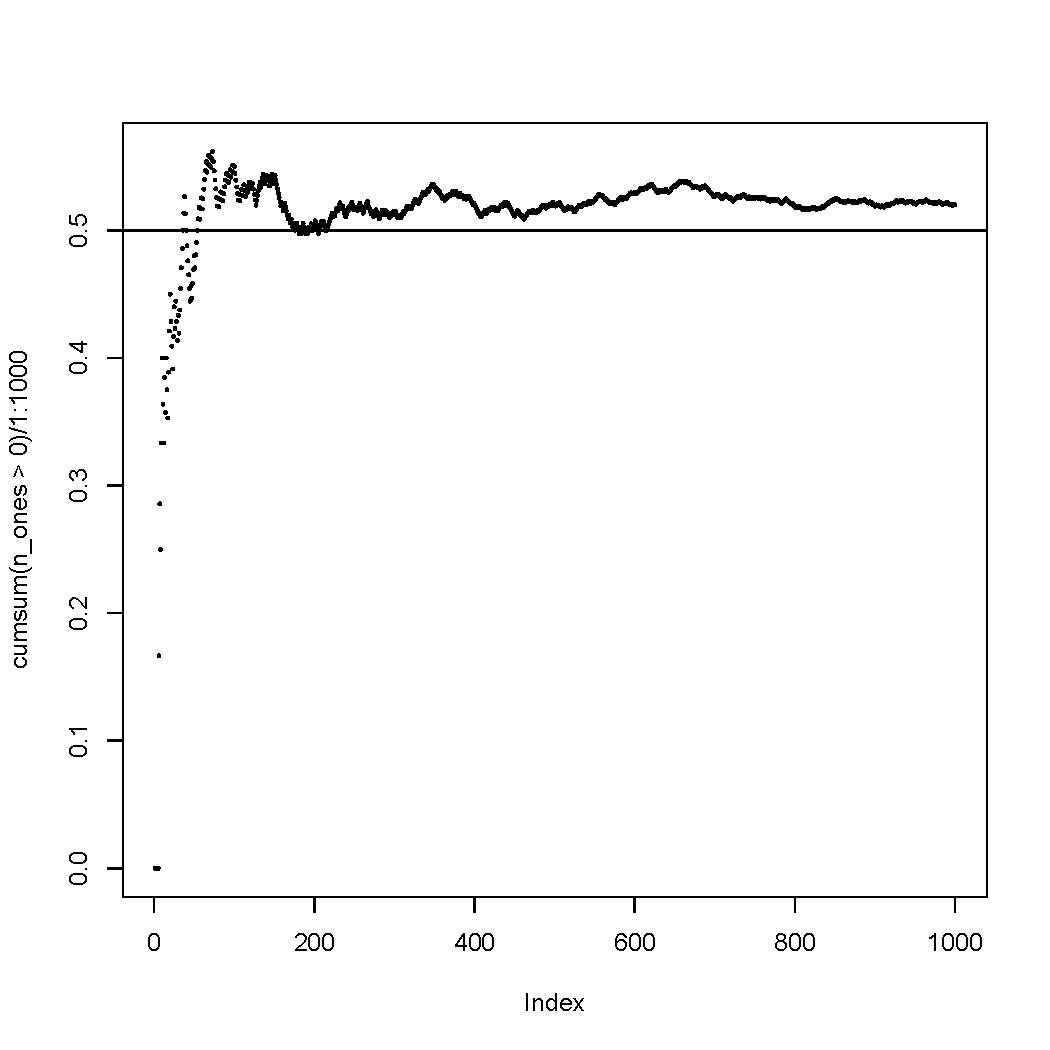
\includegraphics[width=2.7 in]{Plot1.pdf}

\end{frame}

\begin{frame}[fragile]
\begin{verbatim}
> twodice <- outer(1:6, 1:6, paste) # Outcomes for two dice
> twodice24x <- replicate( n = 1000, 
sample(twodice, size = 24, replace=TRUE))
> n_doubleones <- colSums(twodice24x=="1 1")
\end{verbatim}
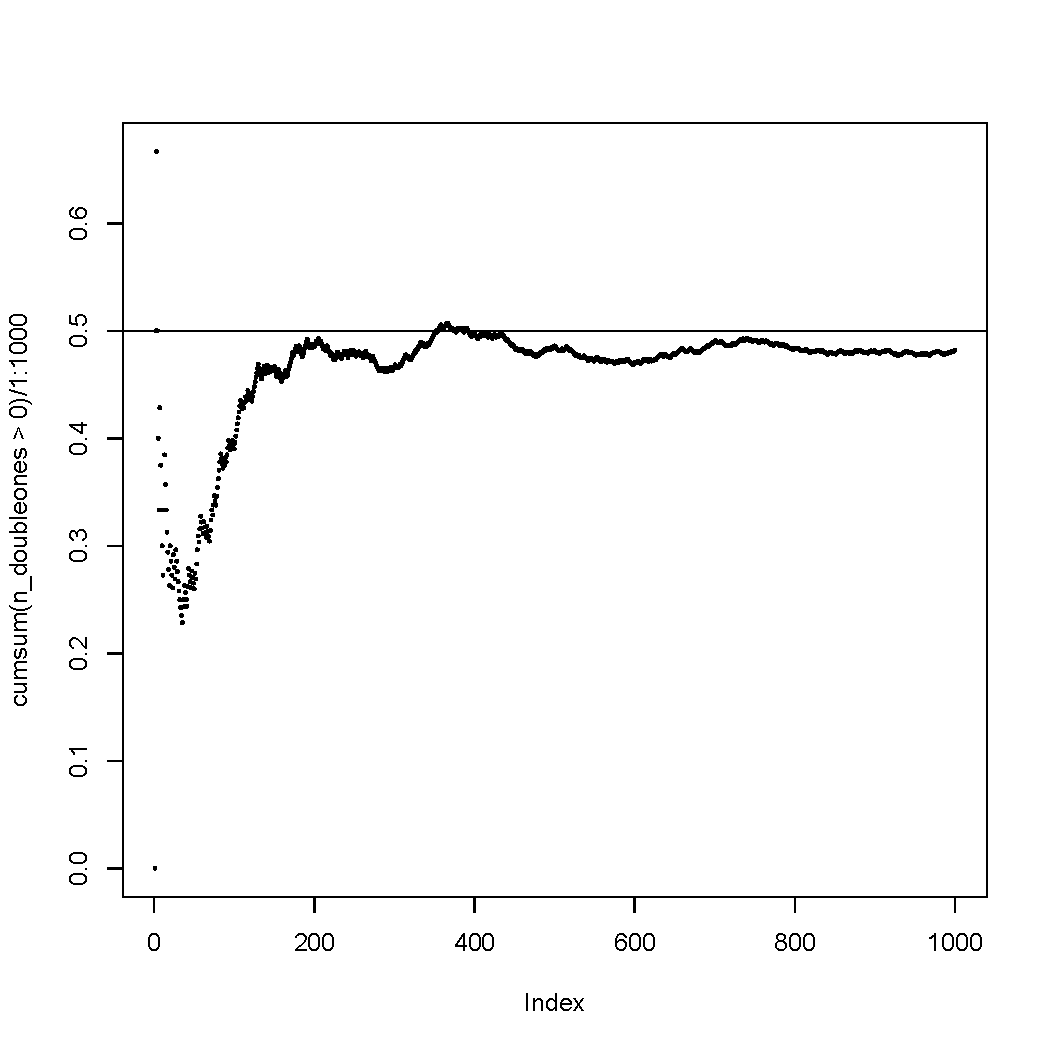
\includegraphics[width=2.7 in]{Plot2.pdf}


\end{frame}


\begin{frame}{Where did Antoine go wrong?}
\begin{itemize}
\item P(two `1` in one roll) is 1/6 as likely as P(one `1' in one roll):
\begin{itemize}
\item One roll, one die = $\{1, 2, 3, 4, 5, 6\} \rightarrow 1/6$
\item One roll, two die = $\{(1,1), (1, 2), (1,3), (1,4), (1,5), (1,6), (2,1),(2, 2),$
\item[] $(2,3), (2,4), (2,5), (2,6), (3,1), (3, 2), (3, 3), ... (6,6)\} \rightarrow 1/36$\pause
\end{itemize}
\item Using these enumerated possibilities, we can calculate probabilities.  
\end{itemize}
\pause
Much of probability is about reasoning backward. \\
\end{frame}


\begin{frame}{Solving by enumeration}
\begin{itemize}
\item[] Roll a die 4 times, the total number of possible outcomes:\\ $6\ \times 6\ \times 6\ \times 6 = 1296$\pause
\item[] Of these, there are 625 outcomes \textbf{without} a `1`:\\  $5\ \times 5\ \times 5\ \times 5 = 625$\pause
\item[] So, Antoine wins bet A 
$$P(A)= \frac{1296-624}{1296} \approx 0.52$$
\end{itemize}
\end{frame}


\begin{frame}{Using Probabilistic Reasoning}
So how about when there are 24 rolls?\\
\vspace{1 cm}
\pause
\vspace{1 cm}
P(no '1' in 4 rolls)$ = (5/6)*(5/6)*(5/6)*(5/6)=(5/6)^4$

$$P(A) = 1- (5/6)^4\approx .52$$
\pause

\vspace{1 cm}

P(no double '1' in 24 rolls)$ = (35/36)^{24}$
$$P(B)=1-(35/36)^{24} \approx .49$$
\end{frame}


\begin{frame}
\frametitle{Sets and Probability}

Probability model represent random phenomenon using mathematical set notation:\pause 
\begin{itemize}
\invisible<1>{\item[1)] Sample space: \{all possible outcomes\}} \pause 
\invisible<1-2>{\item[2)] Events: subsets of the sample space} \pause 
\invisible<1-3>{\item[3)] Probability Law: chance of an event, a non-negative number P(A), where A is some event} 
\end{itemize}
\end{frame}


\begin{frame}
\frametitle{Sample Spaces: All Things that Can Happen}

\begin{defn}
The \alert{sample space} is the set of all things that can occur.  This set is often referred to by the symbol $\Omega$ or $S$.
\end{defn}
\pause 
{Examples: } \pause 
\begin{itemize}
\item[1)] The outcome of two dice  \pause
\begin{itemize}
\item[-] $\Omega = \{`1\ 1', `1\ 2' , `1\ 3', \hdots, `6\ 6'\}$ \pause
\end{itemize}
\item[2)] Survival of Monarch \pause
\begin{itemize}
\item[-] $\Omega = \{t: 0\leq t \leq 120\}$ 
\end{itemize}

\end{itemize}
\end{frame}





\begin{frame}
\frametitle{Events: Subsets of Sample Space}

Events are \alert{sets}\pause\invisible<1>{: collection of distinct
  objects. }  \\
\begin{itemize}
\invisible<1-2>{\item[] $A = \{(Sanders, Ellison), (McMullin, Pence)\}$ } \pause
\invisible<1-3>{\item[] $B  = \{ (Trump, Pence), (Trump, Duke), (McMullin, Pence)\} $} \pause
\invisible<1-4>{\item[] $\Omega = \{ (Trump, Pence), (Sanders, Ellison), (Trump, Duke),$\\ $(McMullin, Pence), (Booker, Harris) \}$} \pause
\invisible<1-5>{\item[] $A\subset \Omega,\ B\subset \Omega, \Omega \subseteq \Omega$} \pause
\end{itemize}
\invisible<1-6>{We can make a new set $E$, using \emph{set operations}} \pause
\begin{itemize}
\invisible<1-7>{\item[1)] Union: $\cup$ } \pause
\begin{itemize}
\invisible<1-8>{\item[-] All objects that appear in \alert{either} set } \pause
\invisible<1-9>{\item[-] $E = A\cup B  = \{(Trump, Pence), (Sanders, Ellison), (Trump, Duke), (McMullin, Pence)\} $} \pause
\end{itemize}
\invisible<1-10>{\item[2)] Intersection: $\cap$ } \pause
\begin{itemize}
\invisible<1-11>{\item[-] All objects that appear in \alert{both} sets } \pause
\invisible<1-12>{\item[-] $F= A\cap B = \{(McMullin, Pence)\} $} \pause
\invisible<1-13>{\item[-] Sometimes written as $AB$} \pause
\end{itemize}
\end{itemize}

\end{frame}


\begin{frame}

\begin{itemize}
\item[3)] \alert{Compliment} of set $E$: $E^{c}$ \pause
\begin{itemize}
\invisible<1>{\item[-] All objects in $\Omega$ that aren't in $E$} \pause
\invisible<1-2>{\item[-] $A^{c} = \{(Trump, Pence), (Trump, Duke),(Booker, Harris) \} $} \pause
\invisible<1-3>{\item[-] $B^{c} = \{(Sanders, Ellison),(Booker, Harris)\} $} \pause 
\invisible<1-4>{\item[-] If $\Omega = \Re$ and $E = [0,1]$.  What is $E^{c}$? } \pause
\invisible<1-5>{\item[-] What is $\Omega^{c}$}? 
\end{itemize}
\end{itemize}


\invisible<1-6>{Suppose $E = \{(McMullin, Pence)\}$, $F = \{(Sanders, Ellison)\}$.  Then  $E \cap F = \emptyset$ (there is nothing that lies in both sets)}

\end{frame}


\begin{frame}
\frametitle{Events: Subsets of Sample Space}

\begin{defn}
Suppose $E$ and $F$ are events.  If $E \cap F = \emptyset$ then we'll say $E$ and $F$ are \alert{mutually exclusive}
\end{defn}

\pause 

\begin{itemize}
\invisible<1>{\item[-] Mutual exclusive events cannot mutually occur} \pause 
\invisible<1-2>{\item[-] $E$ and $E^{c}$ are mutually exclusive events} \pause 
\end{itemize}

\begin{itemize}
\invisible<1-3>{\item[-] If Trump wins reelection, Booker will not be president.} \pause 
\invisible<1-4>{\item[-] If E is mutually exclusive of F, If I know that $E$ happened, I can be sure that F did not.} \pause 
\end{itemize}


\end{frame}



\begin{frame}
\frametitle{Events: Subsets of the Sample Space}

\begin{defn}
Suppose we have events $E_{1}, E_{2}, \hdots, E_{N}$.  \\
Define: 
\begin{eqnarray}
\cup_{i=1}^{N} E_{i} & = & E_{1} \cup E_{2} \cup E_{3} \cup \hdots \cup E_{N} \nonumber
\end{eqnarray}
 $\cup_{i=1}^{N} E_{i} $ is the set of outcomes that occur at least once in $E_{1} , \hdots, E_{N}$.  This is like a logical or. \pause \\

\invisible<1>{
Define: 


\begin{eqnarray}
\cap_{i=1}^{N} E_{i} & = & E_{1} \cap E_{2} \cap \hdots \cap E_{N} \nonumber 
\end{eqnarray}
$\cap_{i=1}^{N} E_{i} $ is the set of outcomes that occur in each $E_{i}$.  This is like a logical and.
}

\end{defn}


\end{frame}




\begin{frame}
\frametitle{Conditions for things to be events}


\begin{condition}
$\Omega$ must be an event. \\
\end{condition}

\invisible<1>{We aren't leaving out $\Omega$.}

\begin{condition}
If $A$ is an event, $A^c$ is an event. \\
\end{condition}

\invisible<1-2>{We can't leave the sample space by taking complements}

\begin{condition}
If $A_1,\ A_2,\ A_3$ ... are a countable collection of events, then $\bigcup_{i=1}^\infty A_i$ is an event. \\
\end{condition}

\invisible<1-3>{We cannot leave out combinations of events.}
\invisible<1-4>{}

\end{frame}




\begin{frame}
\frametitle{Probability Law}

\begin{itemize}
\invisible<1-1>{\item \alert{Probability}: chance of event} \pause 
\begin{itemize}
\invisible<1-2>{\item[-] $P$ is a function} \pause 
\invisible<1-3>{\item[-] Domain: all events $E$} \pause 
\invisible<1-4>{\item[-] Range: $0\leq x\leq1$} \pause 
\invisible<1-5>{\item[-] Describes relative likelihood of all $E$
  (events)} 
\invisible<1-6>{}
\end{itemize}
\end{itemize}

\end{frame}

\begin{frame}
\frametitle{Probability Axioms} 


\begin{defn}
All probability functions, $P$, satisfy three axioms: \pause 
\begin{itemize}
\invisible<1>{\item[1)] (Nonnegativity) For every event $A$, \\} \pause 
\invisible<1-2>{$P(A) \geq 0$ } \pause 
\invisible<1-3>{Chances are never negative} \pause 
\invisible<1-4>{\item[2)] (Additivity) For all sequences of mutually exclusive events $E_{1},
  E_{2}, \hdots,E_{N} $ (where $N$ can go to infinity)\\} \pause 
\invisible<1-5>{$P\left(\cup_{i=1}^{N} E_{i}  \right)  =
  \sum_{i=1}^{N} P(E_{i} ) $} 
\invisible<1-6>{\item[3)] (Normalization) $P(\Omega) = 1$ } \pause 
 \invisible<1-7>   {The probability of certain events is 1} \pause 
\invisible<1-8>{} 

\end{itemize}
\end{defn}
\end{frame}


\begin{frame}
\frametitle{Probability Examples}

\pause 

\begin{itemize}
\invisible<1>{\item[-] Suppose we are flipping a \alert{fair} coin.  Then $P(\{H\}) = P(\{T\}) = 1/2 $}\pause 
\invisible<1-2>{\item[-] Suppose we are rolling a six-sided die.  Then $P(\{1\}) = 1/6$} \pause 
\invisible<1-3>{\item[-] Suppose we are flipping a pair of fair coins.  Then $P(\{(H, H)\}) = 1/4$} 
\end{itemize}

\end{frame}

\begin{frame}
\frametitle{Properties of Probability}

\pause 

\begin{itemize}
\invisible<1>{\item[-] If $A\subseteq B, P(A)\leq P(B) $}\pause 
\invisible<1-2>{\item[-] $P(A\cup B)= P(A)+P(B)-P(A\cap B)$ } \pause 
\invisible<1-3>{\item[-] $P(A\cup A^{c}) = 1$} 
\invisible<1-3>{\item[-] $P(A\cap A^{c}) = 0$} 
\invisible<1-3>{\item[-] $P(\emptyset) = 0 $ } 
\invisible<1-3>{\item[-] $P(E) = 1 - P(E^{c})  $} 
\end{itemize}

\end{frame}

\begin{frame}
\frametitle{Properties of Probability: Monotonicity} 
\pause 
\invisible<1>{\begin{prop} 
If $E \subset F$ then $P(E) \leq P(F)$.  
\end{prop} } \pause 
\invisible<1-2>{\begin{proof} } \pause 
\invisible<1-3>{We can write $F = E \cup ( E^{c} \cap F)$. (Why?) \\} \pause 
\invisible<1-4>{Further, $E\cap(E^{c} \cap F )= \emptyset$ \\}
\pause 
\invisible<1-5>{Then \\} \pause 
\invisible<1-6>{$P(F) = P(E) + P(E^{c} \cap F) $ } \pause 
\invisible<1-7>{\end{proof} }
\invisible<1-7>{As you add more ``outcomes''  to a set, it can't reduce the
probability.  } 
\end{frame}



\begin{frame}
\frametitle{Properties of Probability} 
\begin{prop}
Consider events $E_{1}$ and $E_{2}$.  Then 
\begin{eqnarray}
P(E_{1} \cap E_{2} ) & = & P(E_{1} ) - P(E_{1} \cap E_{2}^{c}) \nonumber 
\end{eqnarray}
\end{prop}

\pause 
\begin{proof}
\begin{eqnarray}
\invisible<1>{E_{1} & = & (E_{1} \cap E_{2}) \cup (E_{1} \cap E_{2}^{c}) \nonumber \\} \pause 
\invisible<1-2>{P(E_{1}) & = & P(E_{1} \cap E_{2} )  + P(E_{1} \cap E_{2}^{c} ) \nonumber \\ } \pause 
\invisible<1-3>{P(E_{1} \cap E_{2} ) & = &  P(E_{1} ) - P(E_{1} \cap E_{2}^{c} ) \nonumber } 
\end{eqnarray}




\end{proof}


\end{frame}


\begin{frame}{Counting and the binomial formula}
If we have $m$ elements, ${{m}\choose{k}}$ is number of ways to choose a subset of size $k$.\\
If we have $m$ sequences of binary outcomes, ${{m}\choose{k}}$ is number of sequences that contain $k$ successes.\\
$${{m}\choose{k}}\equiv\frac{m!}{k!(m-k)!}$$
$$i!\equiv1\cdot2\cdot\cdot\cdot(i-1)\cdot i$$

\pause
Binomial Theorem: 
$$(x+y)^2= x^2+2xy+y^2$$
$$(x+y)^3= x^3+3x^2y+3xy^2+y^3$$
$$(x+y)^4= x^4+4x^3y+6x^2y^2+4xy^3+y^4$$
$...$
$$(x+ y)^{n} = \sum_{i=0}^{n} {{n}\choose {i}} (x)^{n- i} y^{i} $$
\end{frame}



\begin{frame}{Examples of counting}
\begin{itemize}
\item How many different combinations can occur when we throw two dice (ignoring order)?
\item The number of elements $m = 6$ , the subset is size $k=2$\pause
$${{m}\choose{k}}=\frac{6!}{2!(6-2)!}$$\pause
$$=\frac{6\times5\times4\times3\times2}{2\times4\times3\times2}$$
$$=\frac{6\times5}{2}=15$$
\end{itemize}
\end{frame}


\begin{frame}{Examples of counting}
\begin{itemize}
\item How many different networks can occur if there are 24 people?\pause
\item A network is characterized by the presence or absence of a connection (edge) between people (nodes).\pause
\item If there are m nodes, there are ${{m}\choose{2}}=\frac{m!}{2!(m-2)!}=m(m-1)/2$ edges in a complete graph.\pause
\item Each of these edges may be present or absent, so there are two possibilities for each edge, so in if $m=6$:
$$2*2*2*2*2*2*2*2*2*2*2*2*2*2*2=2^{15}=32,768$$
\item If $m=24$, the possibilities are $2^{\frac{24*23}{2}}=2^{276}$\pause
\item For comparison, there are $2^{265}$ atoms in the universe.
\end{itemize}
\end{frame}



\begin{frame}{Examples of counting}
\begin{itemize}
\item How many observations are there in the MIDs dataset?\pause
\item There are about 180 countries in the world.
\item The number of undirected dyads is therefore ${{180}\choose{2}}=16,110$ 
\item The number of directed dyads (where order matters) is twice this.
\item How about when you have four-digit trade data? ${{180*9999}\choose{2}}=1,600,000,000,000$
\end{itemize}
\end{frame}


\begin{frame}{Example of binomial}
\begin{itemize}
\item Suppose we shuffle a 52 card deck and begin flipping over the cards.  What is the probability that the 13 card is the first King?\pause
\item If there is exactly one King in the first thirteen cards, the probability that it is number 13 is 1/13. \pause
\item So what are the chances of assembling 13 cards with one king in them?  Lets compare the total possibilities to the number of successes.\pause 
\begin{itemize}
\item How many total ways are there of getting 13 cards out of 52? \pause \invisible<1-4>{ ${52\choose 13}$}\pause
\item There are 4 kings, so there are four ways to get that 13th card to be a king. \pause
\item How about the 12 cards that are not kings?  \pause \invisible<1-7>{ ${48\choose 12}$}
\end{itemize}
\item \pause \invisible<1-8>{ So the probability is $\frac{1}{13}\cdot \frac{4\cdot{48\choose 12}}{{52\choose13}}$}
\end{itemize}

\end{frame}

\begin{frame}[fragile]
\begin{verbatim}
deck <- outer( c("A", 2:10, "J", "Q", "K"), 
		       c("h", "d", "s", "c"), paste0)
Kings <- paste0("K",  c("h", "d", "s", "c"))

trial <- function(){
	first13 <- sample(as.vector(deck), 13)
	Kingisthere <- first13[13] %in% Kings 
	KingisAlone <- !(TRUE %in% (first13[1:12] %in% Kings))
	return(Kingisthere & KingisAlone)
}

out <- replicate(500000, trial())

mean(out)
[1] 0.033804

(1/13)*(4*choose(48,12))/choose(52, 13)
[1] 0.0337575
\end{verbatim}
\end{frame}


\begin{frame}
\frametitle{Inclusion/Exclusion}

\begin{prop} 
Suppose $E_{1}, E_{2}, \hdots, E_{n}$ are events.  Then 

\begin{eqnarray}
P(E_{1} \cup E_{2} \cup \cdots \cup E_{n} ) & = & \sum_{i=1}^{N} P(E_{i} ) - \sum_{i_{1} <i_{2} } P(E_{i_{1}} \cap E_{i_{2} } )+ \cdots \nonumber \\
& & + (-1)^{r+ 1} \sum_{i_{1}<i_{2} < \cdots< i_{r} } P(E_{i_{1}} \cap E_{i_{2}}\cap \cdots \cap E_{i_{r}} ) \nonumber \\
& & + \cdots + (-1)^{n+1} P(E_{1} \cap E_{2} \cap \cdots E_{n} ) \nonumber 
\end{eqnarray}
\end{prop}

\end{frame}


\begin{frame}
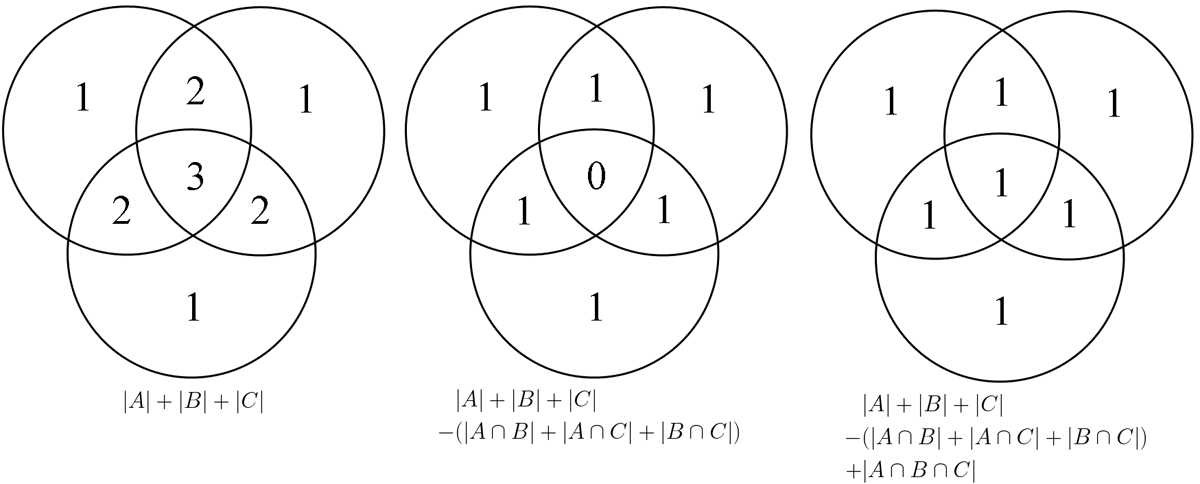
\includegraphics[width=4.8 in]{Inclusion-exclusion-3sets.png}

\end{frame}



\begin{frame}
\frametitle{Proof of Inclusion Exclusion} 

\begin{itemize}
\item[-] Suppose that we have an outcome.  \pause 
\invisible<1>{\item[-] If it isn't in the event sequence, doesn't appear anywhere. }\pause 
\invisible<1-2>{\item[-]  If it is in the event sequence, appears once in $\cup_{i=1}^{n} E_{i}  $, it is in one portion of the Venn diagram, and contributes once to $P(\cup_{i=1}^{n} E_{i})$.   }\pause 
\invisible<1-3>{\item[-] So how do we characterize the addition and subtraction of sets to make it count once?  Suppose it appears in $m$ of the $E_{i}$ $m>0$ }\pause 
\end{itemize}
\begin{eqnarray}
\invisible<1-4>{\text{count} & = & {{m}\choose{1}} - {{m}\choose{2}} + {{m}\choose{3}} - \cdots + (-1)^{m+1} {{m}\choose{m}} \nonumber \\}\pause 
\invisible<1-5>{\text{count} & = & \sum_{i=1}^{m} {{m}\choose{i} } (-1)^{i+1} \nonumber \\}\pause 
\invisible<1-6>{\text{count} & = &  - \sum_{i=1}^{m} {{m}\choose{i} } (-1)^{i} \nonumber  }
\end{eqnarray} 



\end{frame}


\begin{frame}
\frametitle{Proof of Inclusion Exclusion} 

$\text{count}  =   - \sum_{i=1}^{m} {{m}\choose{i} } (-1)^{i}$\\ \pause 
\invisible<1>{Binomial Theorem: $(x+ y)^{n} = \sum_{i=0}^{n} {{n}\choose {i}} (x)^{n- i} y^{i} $.} \pause 
\begin{eqnarray}
\invisible<1-2>{0 = (1 -1 )^m & = & \sum_{i=0}^{m} { {m}\choose{i} } (1)^{m-i}(-1)^{i} \nonumber \\} \pause 
\invisible<1-3>{0 & = & {{m} \choose{0}}(-1)^0 + \sum_{i=1}^{m} {{m} \choose{i}} (-1)^{i} \nonumber \\}  \pause 
\invisible<1-4>{0 & = & 1 + \sum_{i=1}^{m} {{m} \choose{i}} (-1)^{i} \nonumber \\} \pause 
\invisible<1-5>{0 & = & 1 - \text{count} \nonumber \\} \pause 
\invisible<1-6>{1 & = & \text{count} \nonumber } 
\end{eqnarray}


\end{frame}


\begin{frame}
\frametitle{Inclusion/Exclusion}


\begin{cor}
Suppose $E_{1}$ and $E_{2} $ are events.  Then 
\begin{eqnarray}
P(E_{1} \cup E_{2} ) & = & P(E_{1} ) + P(E_{2} ) - P(E_{1} \cap E_{2} ) \nonumber 
\end{eqnarray}
\end{cor}


\end{frame}


\begin{frame}{Relation to Gamma Function}
$${{m}\choose{k}}=\frac{m!}{k!(m-k)!}=\frac{\Gamma(m+1)}{\Gamma(k+1)\Gamma(m-k+1)}$$
If n is an integer:
$$\Gamma(n)=(n-1)!$$
but if z is some real (or complex) number which is not a negative integer:
$$\Gamma(z)=\int_0^\infty x^{z-1}e^{-x}dx$$
$$\Gamma(1)=1$$
$$\Gamma(1/2)=\sqrt{\pi}$$

\end{frame}

\begin{frame}{Why are Gamma Functions useful?}
\begin{itemize}
\item Gamma functions show up in popular distributions: chi-squared distribution, F distribution, and the Students t distribution.
\end{itemize}

\end{frame}



\begin{frame}

\begin{prop}
\alert{Boole's Inequality}
\begin{eqnarray}
P(\cup_{i=1}^{N} E_{i}) & \leq & \sum_{i=1}^{N} P(E_{i} ) \nonumber 
\end{eqnarray}

\end{prop}
\pause 
\invisible<1>{Proof.} \pause \\
\invisible<1-2>{Proceed by induction.  Trivially true for $n =1 $.  Now assume the proposition is true for $n = k$ and consider $n = k + 1$.  } \pause 

\begin{eqnarray}
\invisible<1-3>{P(\cup_{i=1}^{k} E_i \cup E_{k + 1} )  & = & P(\cup_{i=1}^{k} E_i) + P(E_{k + 1} ) - P(\cup_{i=1}^{k} E_i \cap E_{k + 1})\nonumber } \pause 
\end{eqnarray}

\invisible<1-4>{$P(E_{k + 1} ) - P(\cup_{i=1}^{k} E_i \cap E_{k + 1}) \leq P(E_{k + 1} )$\\} 


\end{frame}

\begin{frame}
\frametitle{Proof Continued}

\begin{eqnarray}
P(\cup_{i=1}^{k} E_i ) & \leq  & \sum_{i=1}^{k} P(E_{i} ) \nonumber \\ \pause 
\invisible<1>{P(\cup_{i=1}^{k} E_i) + \alert{P(E_{k + 1} ) - P(\cup_{i=1}^{k} E_i \cap E_{k + 1})} & \leq & 
\sum_{i=1}^{k} P(E_{i} ) + \alert{P(E_{k + 1} )} \nonumber \\} \pause 
\invisible<1-2>{P(\cup_{i=1}^{k + 1} E_i) & \leq & \sum_{i=1}^{k + 1} P(E_{i} )\nonumber} 
\end{eqnarray}



\end{frame}


\begin{frame}

\begin{prop}
Bonferroni's Inequality
\begin{eqnarray}
P(\cap_{i=1}^{n} E_{i} ) & \geq & 1 - \sum_{i=1}^{n} P(E_{i}^{c} ) \nonumber  
\end{eqnarray}

\end{prop}

\pause 
\begin{proof}
\invisible<1>{$\cup_{i=1}^{n} E_{i}^{c} = (\cap_{i=1}^{n} E_{i})^c$.  So, } \pause 
\begin{eqnarray}
\invisible<1-2>{P(\cup_{i=1}^{N} E_{i}^{c} ) & \leq  & \sum_{i=1}^{N} P(E_{i}^{c} ) \nonumber \\} \pause 
\invisible<1-3>{P(\cup_{i=1}^{N} E_{i}^{c} ) & = & P((\cap_{i=1}^{n} E_{i})^c) \nonumber \\
& = & 1 - P(\cap_{i=1}^{n} E_{i}) \nonumber \\} \pause 
\invisible<1-4>{P(\cap_{i=1}^{n} E_{i}) & \geq  &  1- \sum_{i=1}^{n} P(E_{i}^{c} )\nonumber }
\end{eqnarray}



\end{proof}


\end{frame}


\begin{frame}

\begin{defn}
Define the odds of some event $E$ as 
\begin{eqnarray}
\text{odds}_{E} & = & \frac{P(E)}{1 - P(E)} \nonumber 
\end{eqnarray}

Suppose $F$ is another event.  Define the \alert{odds ratio} of E to F as
\begin{eqnarray}
\text{odds ratio}_{E:F} & = & \frac{odds_{E}}{odds_{F}} \nonumber \\
& = & \frac{\frac{P(E)}{1-P(E)}}{\frac{P(F)}{1-P(F)}}\nonumber 
\end{eqnarray}


\end{defn}

\begin{itemize}
\item[-] Big: implies $E$ is very likely
\item[-] Small: implies $E$ is unlikely
\end{itemize}



\end{frame}



\begin{frame}
\frametitle{Uncountable Sample Space} 
\begin{itemize}
\item[] Probability of events on the real line are only positive for intervals.
\item Let $E=\{x : x \in(a,\ b)\}$
$$P(E)=\int_{x \in E} f_X(x) dx$$
 \end{itemize}
\end{frame}


\begin{frame}
\frametitle{Note: Zero Probability $\neq$ Impossible} 

\begin{itemize}
\item Suppose we have a continuous sample space.  $\Omega=\{x : x \in [a,b]\}$
\item We could think of human height, the failure rate of a government, or the length of time it takes to get from Mandalay to Bagan on a riverboat.
\item Technically, no individual point in a continuous sample space can have positive probability.  
\end{itemize}
\end{frame}



\begin{frame}
\frametitle{Example} 
\begin{itemize}
\item Buses can range from being 0 to 10 minutes late.  E might be the probability that a bus is more than 8 minutes late.  Suppose that bus times are uniformly distributed:
 $$P(Late)=\int_{8}^{10} f_X(x) dx$$
 $$P(Late)=\int_{8}^{10} \frac{1}{10}dx$$
 $$P(Late)=\frac{10}{10}-\frac{8}{10}=\frac{2}{10}$$
\end{itemize}
\end{frame}



\begin{frame}
\frametitle{Summary of Terms/Concepts}
\begin{itemize}
\item Sample Space, Event, Probability Law
\item 3 Axioms of Probability 
\item Mutually Exclusive Events
\item Uncountable Sample Spaces
\end{itemize}
\end{frame}




\end{document}